%==============================================================================
%== template for LATEX poster =================================================
%==============================================================================
%
%--A0 beamer slide-------------------------------------------------------------
\documentclass[final]{beamer}
\usepackage[orientation=landscape,size=a0,
            scale=1.5        % font scale factor
           ]{beamerposter}
           
\geometry{
  hmargin=2.5cm, % little modification of margins
}

%
\usepackage[utf8]{inputenc}

\linespread{1.15}
%
%==The poster style============================================================
\usetheme{sharelatex}

%==Title, date and authors of the poster=======================================
\title
[Machine Learning 1, Kaiserslautern, Germany ] % Conference
{ % Poster title
Word embeddings for predicting political affiliation based on
Twitter data
}

\author{ % Authors
Ibrahim\inst{1}, Saurabh\inst{1}, Oliver\inst{1}, Venkatesh\inst{1}, Shridhar\inst{1}, Angjela\inst{1}, Shriram\inst{1}
}
\institute
[Technische Universität Kaiserslautern] % General University
{
\inst{1} Technische Universität Kaiserslautern\\[0.3ex]

}
\date{\today}



\begin{document}
\begin{frame}[t]
%==============================================================================
\begin{multicols}{3}
%==============================================================================
%==The poster content==========================================================
%==============================================================================

\section{Introduction}
\begin{itemize}
  \item Plethora of means to communicate political alignment
  \item Twitter, one of the main source containing message specific to general public
  \item Aim is the quantitative analysis of party affiliations of a user
  \item We propose a deep learning based classification model using state-of-the-art word embeddings
\end{itemize}

\section{Data Sets and Feature Extraction}

\subsection{Dataset Collection}
\begin{itemize}
  \item Tweets made by political figures on Twitter
  \item Categorized data set taken from \href{www.wahl.de/politiker}{www.wahl.de/politiker}
  \item Dividing data into train set and test set for supervised learning
\end{itemize}


\subsection{Feature Extraction}
\begin{itemize}
  \item Obtain vector representation of words under some similarity metrics (word embeddings)
  \item WordtoVec using Continuous Bag of Words and Skip Grams
  \item GloVe embeddings performed on global word-word co-occurrence statistics from a corpus
\end{itemize}

\centering
\begin{figure}[h!]
  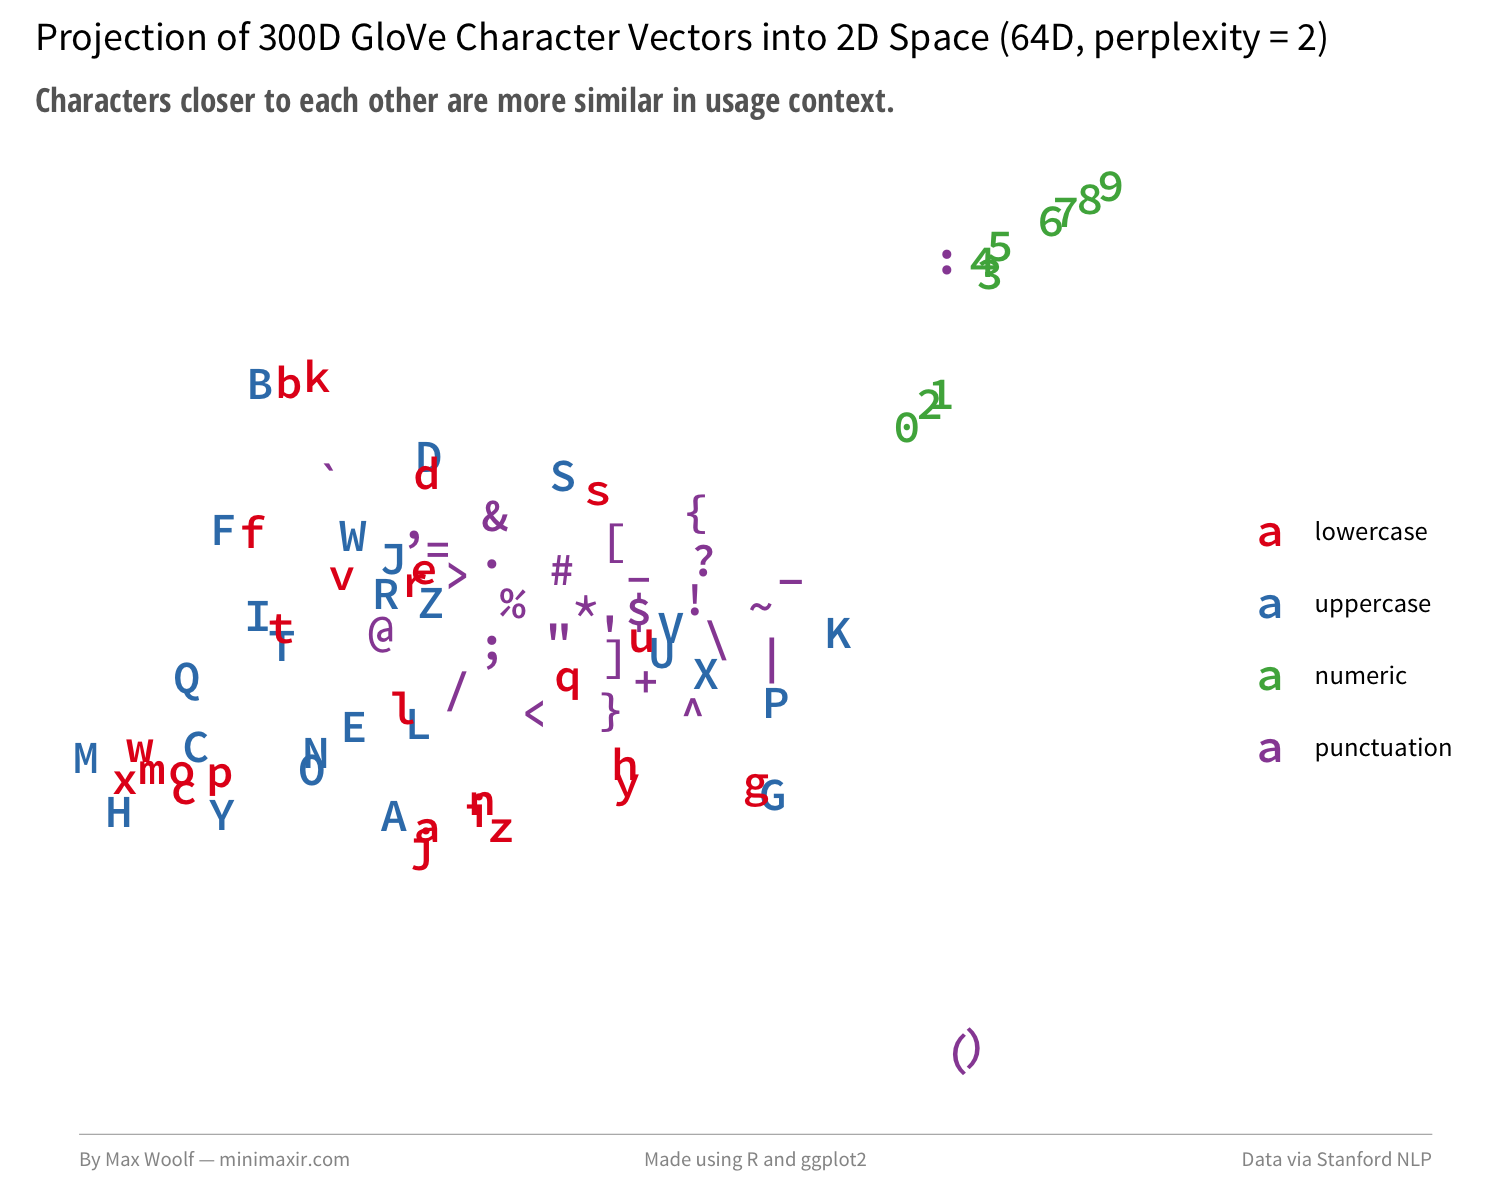
\includegraphics[width=0.70\linewidth]{char-tsne-2.png}
  \label{fig:glove}
\end{figure}


\centering
\begin{figure}[h!]
  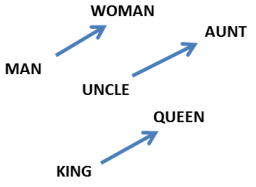
\includegraphics[width=0.30\linewidth]{Vecs}
  \label{fig:glove}
\end{figure}


\section{Recent Developments}
\begin{itemize}
  \item Existing research \cite{ref2} tackle the text classification problem by techniques like SVM, SVD and LSM
  \item Approaches solely considers political affiliations in America, which is relatively easy problem
  \item Many research papers compare different classifiers \cite{ref1}, and do not propose a well-developed solution
  \item Sentiment classification is mostly covered using recurrent- or convolutional neural networks \cite{ref4}
  \item Classifiers cannot be used for classifying users outside the training data.\cite{ref3}
\end{itemize}
\centering
\centering
\begin{figure}[h!]
  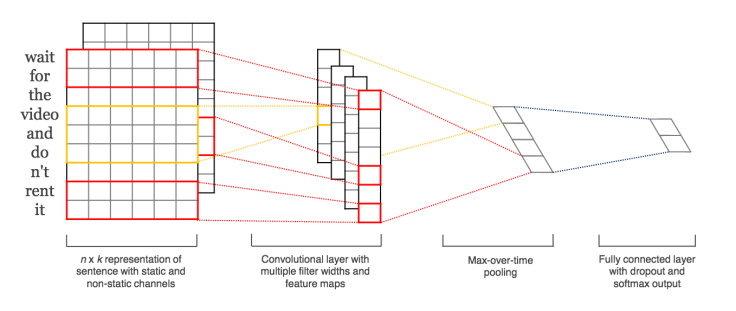
\includegraphics[width=0.90\linewidth]{cnn.png}
  \label{fig:embedding}
\end{figure}


\section{Proposed Methodology}

\begin{itemize}
  \item Using a CNN to learn features from different word-lengths for classification
  \item Use bi-directional LSTM, which caters the need to learn the context in temporal space
  \item Idea is to use a combination of above approaches in an end-to-end learning
\end{itemize}

\section{Analysis of Results}
\begin{itemize}
    \item Quantitative analysis of result under various metrics like F1-score, cross-entropy logarithmic loss
    \item Visual analysis of embedding space and results using T-SNE or PCA
\end{itemize}

%==============================================================================
%==End of content==============================================================
%==============================================================================

%--References------------------------------------------------------------------

\subsection{References}
\begin{thebibliography}{99}
\bibitem{ref1} Maneesh Bhanda, Dan Robinson, and Conal Sathi. Text classifiers for political accuracy that they report, it is stated that the ideologies. 2009.
\bibitem{ref2} Felix Biessmann, Pola Lehmann, Daniel Kirsch, and Sebastian Schelter. Predicting political party affiliation from text. 2017.
\bibitem{ref3} Raviv Cohen and Derek Ruths. Classify-ing political orientation on twitter: It’s not easy!
\bibitem{ref4} Yoon Kim. Convolutional neural networks for sentence classification

\end{thebibliography}
\end{multicols}

%==============================================================================
\end{frame}
\end{document}
